\section{Lifecycle}
\label{subsec:high_level_lifecycle}
It was decided early that the new ECS would follow a lifecycle akin to the one in the existing NOX Actor system,
which was inspired by the Android activity lifecycle\cite{android_activity_lifecycle}.

The new ECS lifecycle borrows heavily from the NOX Actor system's lifecycle, with some minor name changes,
and the addition of the raw memory stage, to clear up certain confusions with the previous lifecycle.
Just as within the NOX Actor system, a component can go through different stages of a lifecycle during its lifetime.
The lifecycle allows the users to release unnecessary resources when a component is in a more inactive stage.
The following sections describe each stage in the entity lifecycle.
The lifecycle and its corresponding transitions can be seen in figure \ref{fig:lifecycle}.

\subsection{Raw Memory Stage}
Unlike the other parts of the lifecycle, raw memory is not a stage that a component can actually be in,
as this stage is before a constructor has been run on an object.
The rationale for this stage is to clear up any confusion within the old NOX Actor system,
in relation to what happens to an object that has been destroyed.
Within the old NOX Actor system an object that had been destroyed could still be brought back to life,
meaning that a destroyed object was per definition still alive.
The destroyed stage were renamed to hibernation, and the raw memory stage was added.
Since the NOX ECS is pooling and reusing its memory, it needs to be clear that when we discuss objects
that has been destructed, that object is destructed in the sense that it is now just raw memory.
At this point nothing is know about the object, so a component that has been turned into raw memory cant be rebuilt.

\subsection{Hibernation Stage}
Hibernation is the first stage within the lifecycle where a component can be said to be valid.
This stage is either directly after the constructor or after an user requested initialize function has been executed on a component.
The stage is meant to be used when a component will be inactive for a longer period of time, similarly to "Stopped" in the Android Activity State\cite[Activity state and ejection from memory]{android_activity_lifecycle}.
A component that is hibernating should only contain it's most basic resources, to not waste space or time within the program.

\subsection{Inactive Stage}
Inactive is meant for short term component inactivity.
A component that is inactive should hold on to most of it's resources, allowing for reactivation to be a lightweight transition.
Within the Android Activity States this would be the "Paused" state\cite[Activity state and ejection from memory]{android_activity_lifecycle}.

\subsection{Active Stage}
A component that is active is one that is currently running within the system.
This component has all its resources available and is currently getting its update function called.

\subsection{Stage Transitions}
Components transition through the different stages of a lifecycle through transition requests via function calls.
Transitions are handled asynchronously, however multiple transitions will by default be executed together.
This means that one can request a component to awake and activate, and this will still by default only take one frame.
The transitions are as follows.
\begin{description}
    \item
    [Awake] Transitions a component from the hibernation stage to the inactive stage.

    \item
    [Activate] Transitions a component from the inactive stage to the active stage.

    \item
    [Deactivate] Transitions a component from the active stage to the inactive stage.

    \item
    [Hibernate] Transitions a component from the inactive stage to the hibernation stage.
\end{description}

Unlike within the Android lifecycle model, the new ECS will not eject objects from memory based on their lifecycle stage\cite[Activity state and ejection from memory]{android_activity_lifecycle}.
The system does not have enough information regarding the importance of objects, neither how to recreate them from their different stages.
Implementing a lifecycle was done to allow the user of the system better control over resource usage, both in terms of memory
and in terms of computation, as certain functions will not be called on objects based on their stage in the lifecycle.
As a result of this components are not allowed to skip stages in the lifecycle, as that would invalidate invariants within the ECS.

\begin{figure}[tbp]
    \begin{center}
    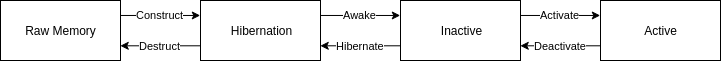
\includegraphics[scale=0.5]{images/lifecycle_horizontal.png}
    \caption{Lifecycle}
    \label{fig:lifecycle}
    \end{center}
\end{figure}
